\section{Modeling Edit Distance}\label{sec:apdx:model_distance}
This section presents our hierarchical Bayesian approaches for analyzing the edit distance data. We first describe a model for edit distance per option (\Cref{sec:apdx:model_distance_option}), followed by analysis for edit distance per action (\Cref{sec:apdx:model_distance_variance}). Finally, we detail a model for cumulative edit distances (\Cref{sec:apdx:model_cum_distance}).

\subsection{Model 1: Edit Distance per Option} \label{sec:apdx:model_distance_option}

\subsubsection{Likelihood}
The dependent variable in this model is the edit distance accumulated for each option, denoted by $D_i$, where $i$ refers to the $i$-th observation. Since $D_i$ must be positive, we model it using an exponential likelihood:

\begin{equation}\label{eq:distance_model_1_likelihood}
D_i \sim \text{Exponential}\bigl(\text{scale} = \lambda_i\bigr).
\end{equation}

\subsubsection{Independent variables and regression model}
We designed $\eta_i$ as the linear predictor that informs $D_i$ through the following transformation:
\begin{equation}\label{eq:transformation_model_1}
\lambda_i = \exp(\eta_i),
\end{equation}
where $\lambda_i$ is the scale (i.e., mean) parameter of the Exponential distribution, and thus must be positive.

This linear predictor:
\begin{equation}\label{eq:distance_model_1_eta}
    \eta_i = \gamma_i + \beta_I[I_i] + \phi_{ij} + U_i
\end{equation}
consists of four components: the length of the option $L_i$, interface type $I_i$, and interaction effect between both length and interface $\phi_{ij}$, and user effect $U_i$ which we describe in the following paragraphs.

\paragraph{Length.} Since length has two levels (short and long), we define:
\begin{equation}
    \gamma_i = \mu_L + \beta_L \cdot L_i 
    \label{eq:distance_model_1_eta_ordinal}
\end{equation}
where $L_i \in \{0,1\}$, making $\gamma_i = \mu_L$ for the short condition and $\gamma_i = \mu_L + \beta_L$ for the long condition. We assign standard normal priors to these parameters: $\mu_L \sim \mathcal{N}(0,1)$ and $\beta_L \sim \mathcal{N}(0,1)$. 

\paragraph{Interface.}
We model the interface effects using a non-centered parameterization to improve numerical stability and encourage partial pooling across the two interface levels. Specifically we let $\mu_{\beta_I} \sim \mathcal{N}(0,1)$ and $\sigma_{\beta_I} \sim \mathrm{HalfNormal}(0.5)$ represent the shared mean and scale of the interface effects. We then sample a raw effect vector $\beta_{I_{\text{raw}}} \sim \mathcal{N}(0,1)^2.$ Combining these, we define:
\begin{equation}
    \beta_I = \mu_{\beta_I} + \sigma_{\beta_I} \cdot \beta_{I_{\text{raw}}}
    \label{eq:distance_interface_reparam}
\end{equation}
where $\beta_I \in \mathbb{R}^2$ contains the effect for each of the two interface levels, 
and $\beta_I[I_i]$ indexes the effect for participant $i$'s interface. 

\paragraph{Interaction Effects} To capture potential interaction effects between length and interface types, we assign one interaction parameter, $\phi_{i,j}$, to each combination of length $i$ ($i \in \{0,1\}$) for short and long surveys and interface $j$ ($j \in \{0,1\}$) for the two interface types. Rather than sampling these $\phi_{i,j}$ directly, we employ a non-centered parameterization:
\[
  \boldsymbol{\phi} = L_{\Omega} \,\bigl(\sigma_{\phi} \odot z_{\phi}\bigr),
\]
where \(\boldsymbol{\phi}\) is a $2 \times 2$ matrix of interaction parameters (since we have 2 levels of length and 2 levels of interface), $z_{\phi} \sim \mathcal{N}(0,1)^{2\times2}$, $\sigma_{\phi} \sim \text{HalfNormal}(0.5)^{2\times2}$, and $L_{\Omega}$ is the Cholesky factor of a $2\times2$ correlation matrix drawn from an $\text{LKJ}(2)$ prior with shape parameter $\eta=3$. We then define
\begin{equation}
    \phi_{ij} = \bigl[\boldsymbol{\phi}\bigr]_{i,j}
\end{equation}
making $\phi_{ij}$ a \emph{single scalar} drawn from the correlated matrix $\boldsymbol{\phi}$.

\paragraph{Individual user effects.} 
Similar to the interface, we also applied a non-centered parameterization to user effects using the same approach:
\begin{equation}\label{eq:distance_model_1_user_effect}
    U_i = \mu_U + \sigma_U \cdot z_U 
\end{equation}

We assign weakly informative priors for the user effects: $\mu_U \sim \mathcal{N}(0,1)$ and $\sigma_U \sim \mathrm{Exponential}(0.5)$, which represent the shared mean and scale of the user effects. We use $z_U \sim \mathcal{N}(0,1)^{40}.$ to denote the $40$ participant's raw user effect vector. This approach allow us to capture user variations across all users.

\subsubsection{Posterior predictive plots}
Our Bayesian model converged successfully, as evidenced by an $\hat{R}$ value of 1 in the model summary. We plotted the posterior predictive distribution for the edit distance per option in Figure~\ref{fig:ppc_distance_m1}. This figure compares the models posterior predictive distribution with the observed data. 

\begin{figure}[h!]
    \centering
    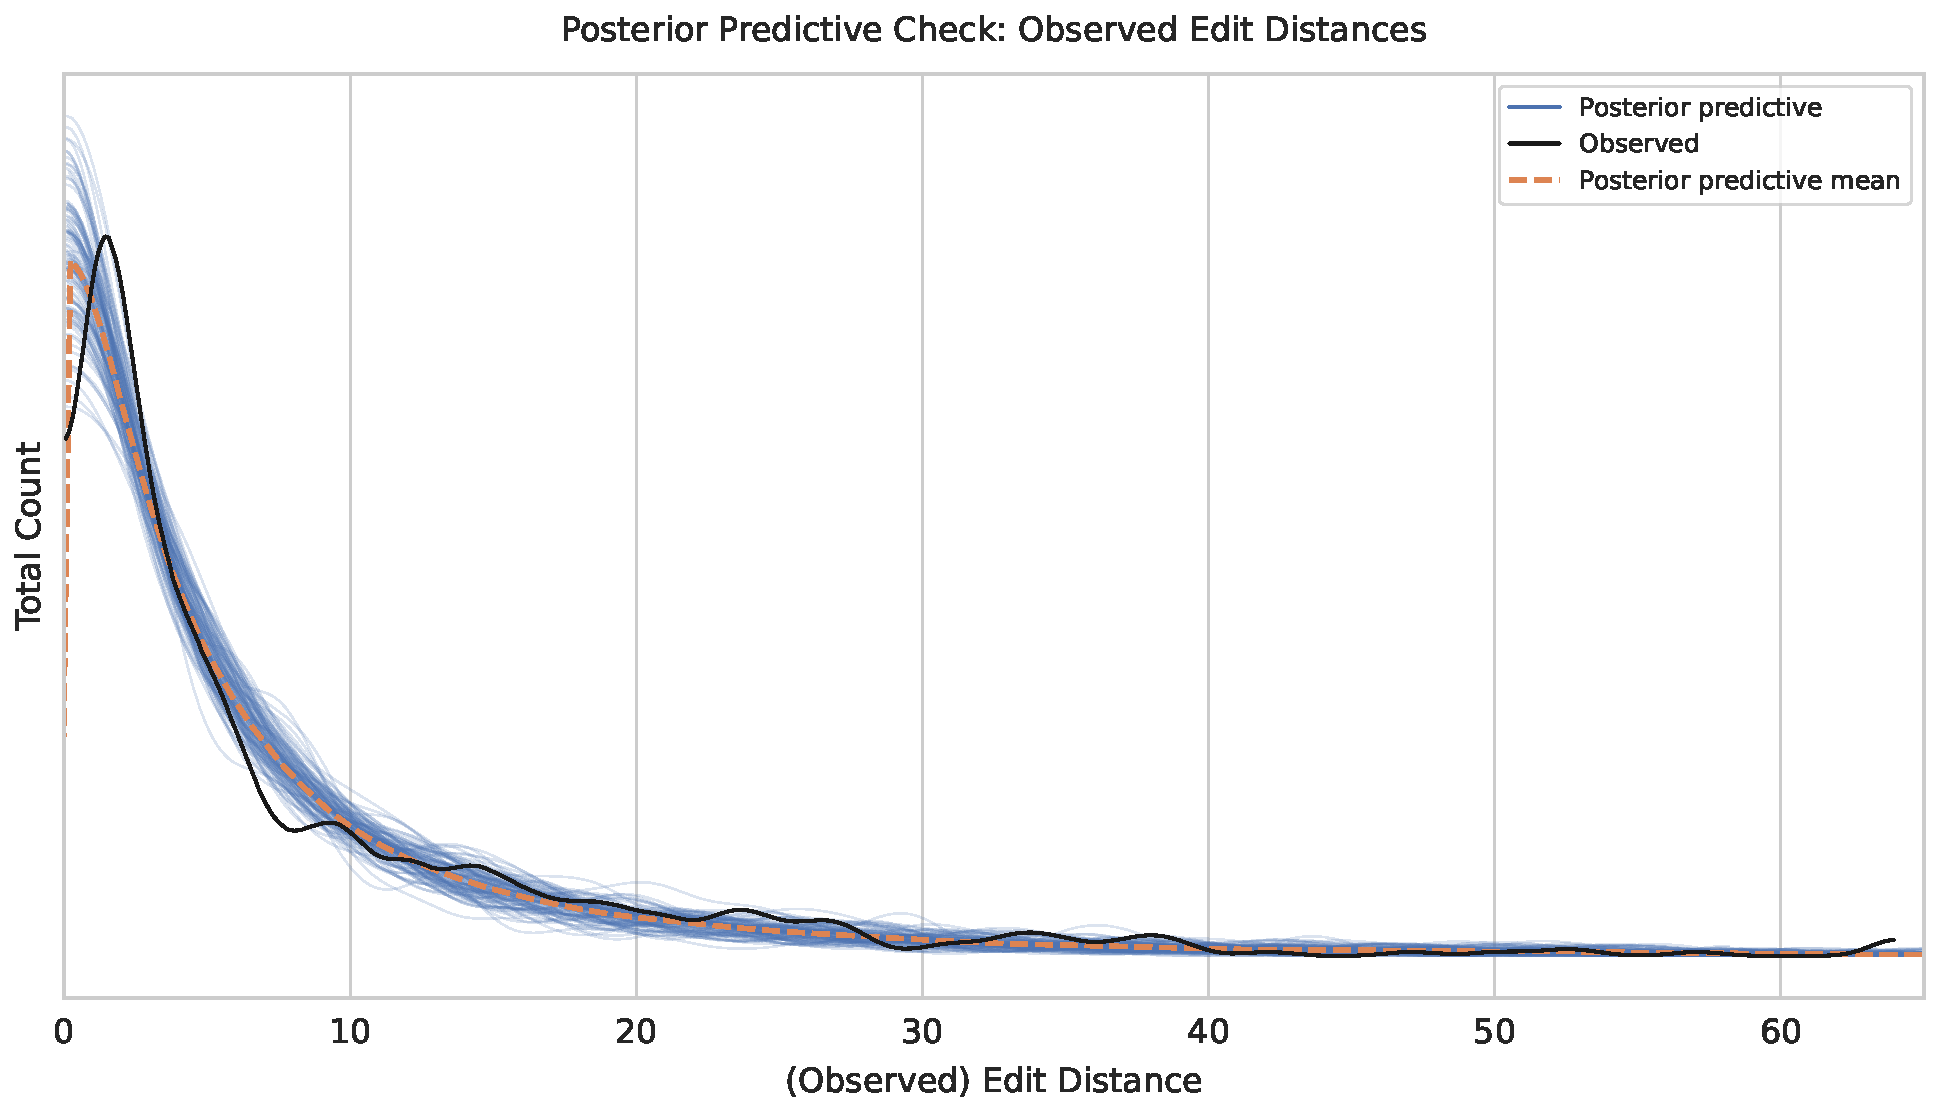
\includegraphics[width=0.45\textwidth]{content/image/distance/ppc_distance_m1.pdf}
    \caption{Posterior Predictions vs. observed data for edit distance per option. Each blue line represents a draw from the posterior distribution, while the black line represents the observed data. Dotted line represents the mean of the posterior data. \textbf{Takeaway of the plot}: We believe that the model is reasonable at capturing the distribution.}
    \Description{ A line plot titled "Posterior Predictive Check: Observed Edit Distances," comparing observed edit distances with model predictions. Multiple thin blue lines indicating individual model simulations. A solid black line representing actual observed data. A dashed orange line showing the average of posterior predictions. The plot illustrates strong alignment between observed data and the posterior predictive mean, with deviations primarily at higher edit distances. This indicates a well-calibrated model fit for most of the distribution.}
    \label{fig:ppc_distance_m1}
\end{figure}

\begin{figure*}[h!]
    \centering
    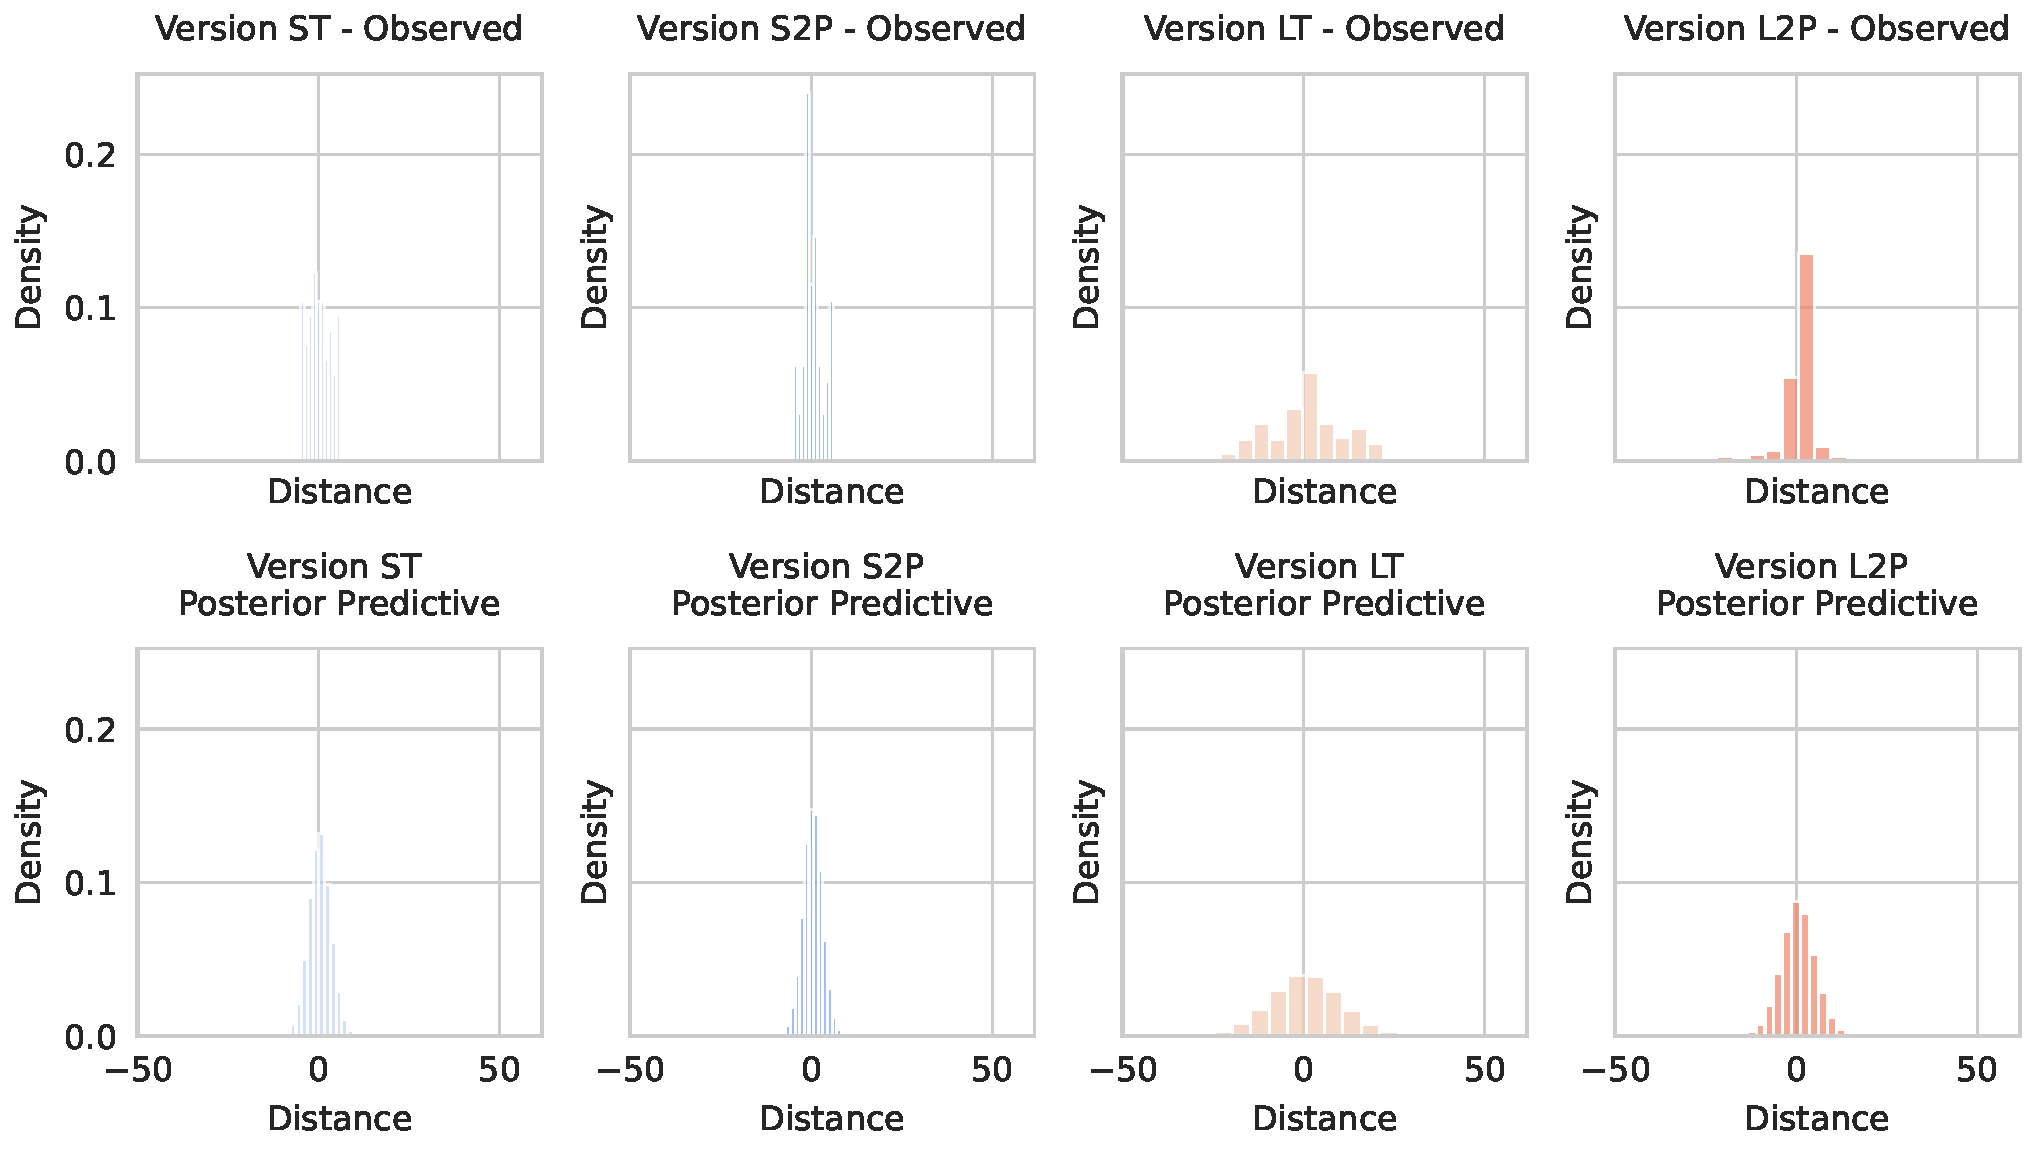
\includegraphics[width=0.75\textwidth]{content/image/distance/observed_vs_posterior_predictive_histogram_m2.pdf}
    \caption{Posterior Predictions vs. Observed Data for Edit Distance per Option. The first row represents the distribution of edit distance per version. The second row shows the posterior predictions after multiple draws \textbf{Takeaway of the plot}: We believe that the model is reasonable at capturing the shape of the distributions though being slightly conservative for extreme values at the center. Future model enhancements could re-model them with a student-t distribution.}
    \Description{
        A grid of eight density plots comparing observed and posterior predictive distributions across four model versions (ST, S2P, LT, L2P). The top row displays observed distributions, and the bottom row displays posterior predictive distributions. Each plot has "Distance" on the x-axis ranging from -50 to 50 and "Density" on the y-axis. Observed distributions are more sparse, while posterior predictive distributions are tightly centered around zero for all model versions. Differences in spread and shape are noticeable, particularly between the LT and L2P models, which show wider and more peaked distributions compared to ST and S2P.
    }

    \label{fig:observed_vs_posterior_predictive_histogram_m2}
\end{figure*}

\subsection{Model 2: Edit Distance with Separate Mean and Variance Predictors} \label{sec:apdx:model_distance_variance}

\subsubsection{Likelihood}
The dependent variable for this model is the edit distance $D_i$, where positive values indicate a downward movement and negative values indicate an upward movement. To allow for different effects on both the mean and variance, we model $D_i$ using a Normal distribution:

\begin{equation}\label{eq:distance_model_2_likelihood}
D_i \sim \mathcal{N}\bigl(\mu_i, \sigma_{\text{obs},i}\bigr)
\end{equation}

\noindent Because our aim is to capture potential differences in variability (e.g., hypothesizing that a two-phase interface might yield lower oscillation than a text-based interface), we separately model both the mean $\mu_i$ and the standard deviation $\sigma_{\text{obs},i}$.

\subsubsection{Independent variables and regression model}

We specify two linear predictors: one for the mean $\mu_i$ (Equation~\ref{eq:distance_model_2_mu}) and one for the (logged) standard deviation $\log(\sigma_{\text{obs},i})$ (Equation~\ref{eq:distance_model_2_sigma}). Both linear predictors incorporate the following factors: the length of the option $L_i$, the interface type $I_i$, an interaction term $\phi_{ij}$, and a user-specific term $U_i$.

\begin{align} 
\mu_i &= \gamma_{\mu,i} + \beta_{I,\mu}[I_i] + \phi_{\mu,ij} + U_{\mu,i}, \label{eq:distance_model_2_mu}\\
log(\sigma_{\text{obs},i}) &= \gamma_{\sigma,i} + \beta_{I,\sigma}[I_i] + \phi_{\sigma,ij} + U_{\sigma,i}. \label{eq:distance_model_2_sigma} 
\end{align}

\paragraph{Length ($L_i$).} Similar to the previous model, we continue to define length as an ordinal value. In this model, the effect for mean and variance are modeled separately. We write: 
\begin{align} 
\gamma_{\mu,i} &= \mu_{L,\mu} + \beta_{L,\mu} \cdot L_i, \label{eq:distance_model_2_gamma_mu}\\
\gamma_{\sigma,i} &= \mu_{L,\sigma} + \beta_{L,\sigma} \cdot L_i. \label{eq:distance_model_2_gamma_sigma} 
\end{align}
For both the mean and variance parts, $\mu_{L,\mu}, \beta_{L,\mu}$ and $\mu_{L,\sigma}, \beta_{L,\sigma}$ capture how option length shifts the location and scale of the distribution, respectively. We assign weakly informative normal priors:
\begin{equation}
    \mu_{L,\mu}, \beta_{L,\mu}, \mu_{L,\sigma}, \beta_{L,\sigma} \sim \mathcal{N}(0, 1).
\end{equation}


\paragraph{Interface ($I_i$).} We treat the interface type as a categorical variable with two levels. As in Model 1, we use a non-centered parameterization for numerical stability and partial pooling. For the mean part, we define: \begin{equation}\label{eq:distance_model_2_beta_I_mu} 
\beta_{I,\mu}[I_i] = \mu_{I,\mu} + \sigma_{I,\mu} \cdot z_{I,\mu}[I_i].
\end{equation} and similarly for the variance part: 
\begin{equation}\label{eq:distance_model_2_beta_I_sigma} 
\beta{I,\sigma}[I_i] = \mu_{I,\sigma} + \sigma_{I,\sigma} \cdot z_{I,\sigma}[I_i].
\end{equation} 

\noindent We place weakly informative priors on the intercepts:
\begin{align}
\mu_{I,\mu}, \beta_{I,\mu}, z_{I,\mu}, \mu_{I,\sigma}, \beta_{I,\sigma}, z_{I,\sigma} \sim \mathcal{N}(0, 1),\\
\sigma_{I,\mu}, \sigma_{I,\sigma} \sim \text{HalfNormal}(0.5).
\end{align}.

\paragraph{Interaction Effects ($\phi_{ij}$).} We hypothesize that the effect of length might vary by interface. Similar to Model 1’s approach, we employ a non-centered parameterization with an LKJ correlation prior. Specifically, for both the mean and variance parts, we define: 
\begin{align} 
\phi_{\mu,ij} &= \bigl[L_{\Omega,\mu},\bigl(\sigma_{\phi,\mu} \odot z_{\phi,\mu}\bigr)\bigr]{i,j}, \label{eq:distance_model_2_phi_mu} \\
phi{\sigma,ij} &= \bigl[L_{\Omega,\sigma},\bigl(\sigma_{\phi,\sigma} \odot z_{\phi,\sigma}\bigr)\bigr]{i,j}, \label{eq:distance_model_2_phi_sigma} 
\end{align} 
where $i \in {0,1}$ (short or long) and $j \in {0,1}$ (two interface types). We continue the use of weakly informed priors:
\begin{align}
z_{\phi,\mu}, z_{\phi,\sigma} \sim \mathcal{N}(0, 1), \sigma_{\phi,\mu}, \sigma_{\phi,\sigma} \sim \text{HalfNormal}(0.5),\\
L_{\Omega,\mu}, L_{\Omega,\sigma} \sim \text{LKJ}(3).
\end{align}

\paragraph{Individual user effects ($U_i$).} To account for participant-level variability, we follow model 1 and adopt a non-centered parameterization but allow each user to have a distinct shift on both $\mu_i$ and $\log(\sigma_{\text{obs},i})$:
\begin{align} 
U_{\mu,i} &= \mu_{U,\mu} + \sigma_{U,\mu} \cdot z_{U,\mu,i}, \label{eq:distance_model_2_user_mu}\\
U_{\sigma,i} &= \mu_{U,\sigma} + \sigma_{U,\sigma} \cdot z_{U,\sigma,i}, \label{eq:distance_model_2_user_sigma}
\end{align} 
with priors:
\begin{align}
    \mu_{U,\mu}, \beta_{U,\mu}, z_{U,\mu,i}, \mu_{U,\sigma}, \beta_{U,\sigma}, z_{U,\sigma,i} \sim \mathcal{N}(0, 1),\\
    \sigma_{U,\mu}, \sigma_{U,\sigma} \sim \text{HalfNormal}(0.5).
\end{align}

\begin{figure*}[h!]
    \centering
    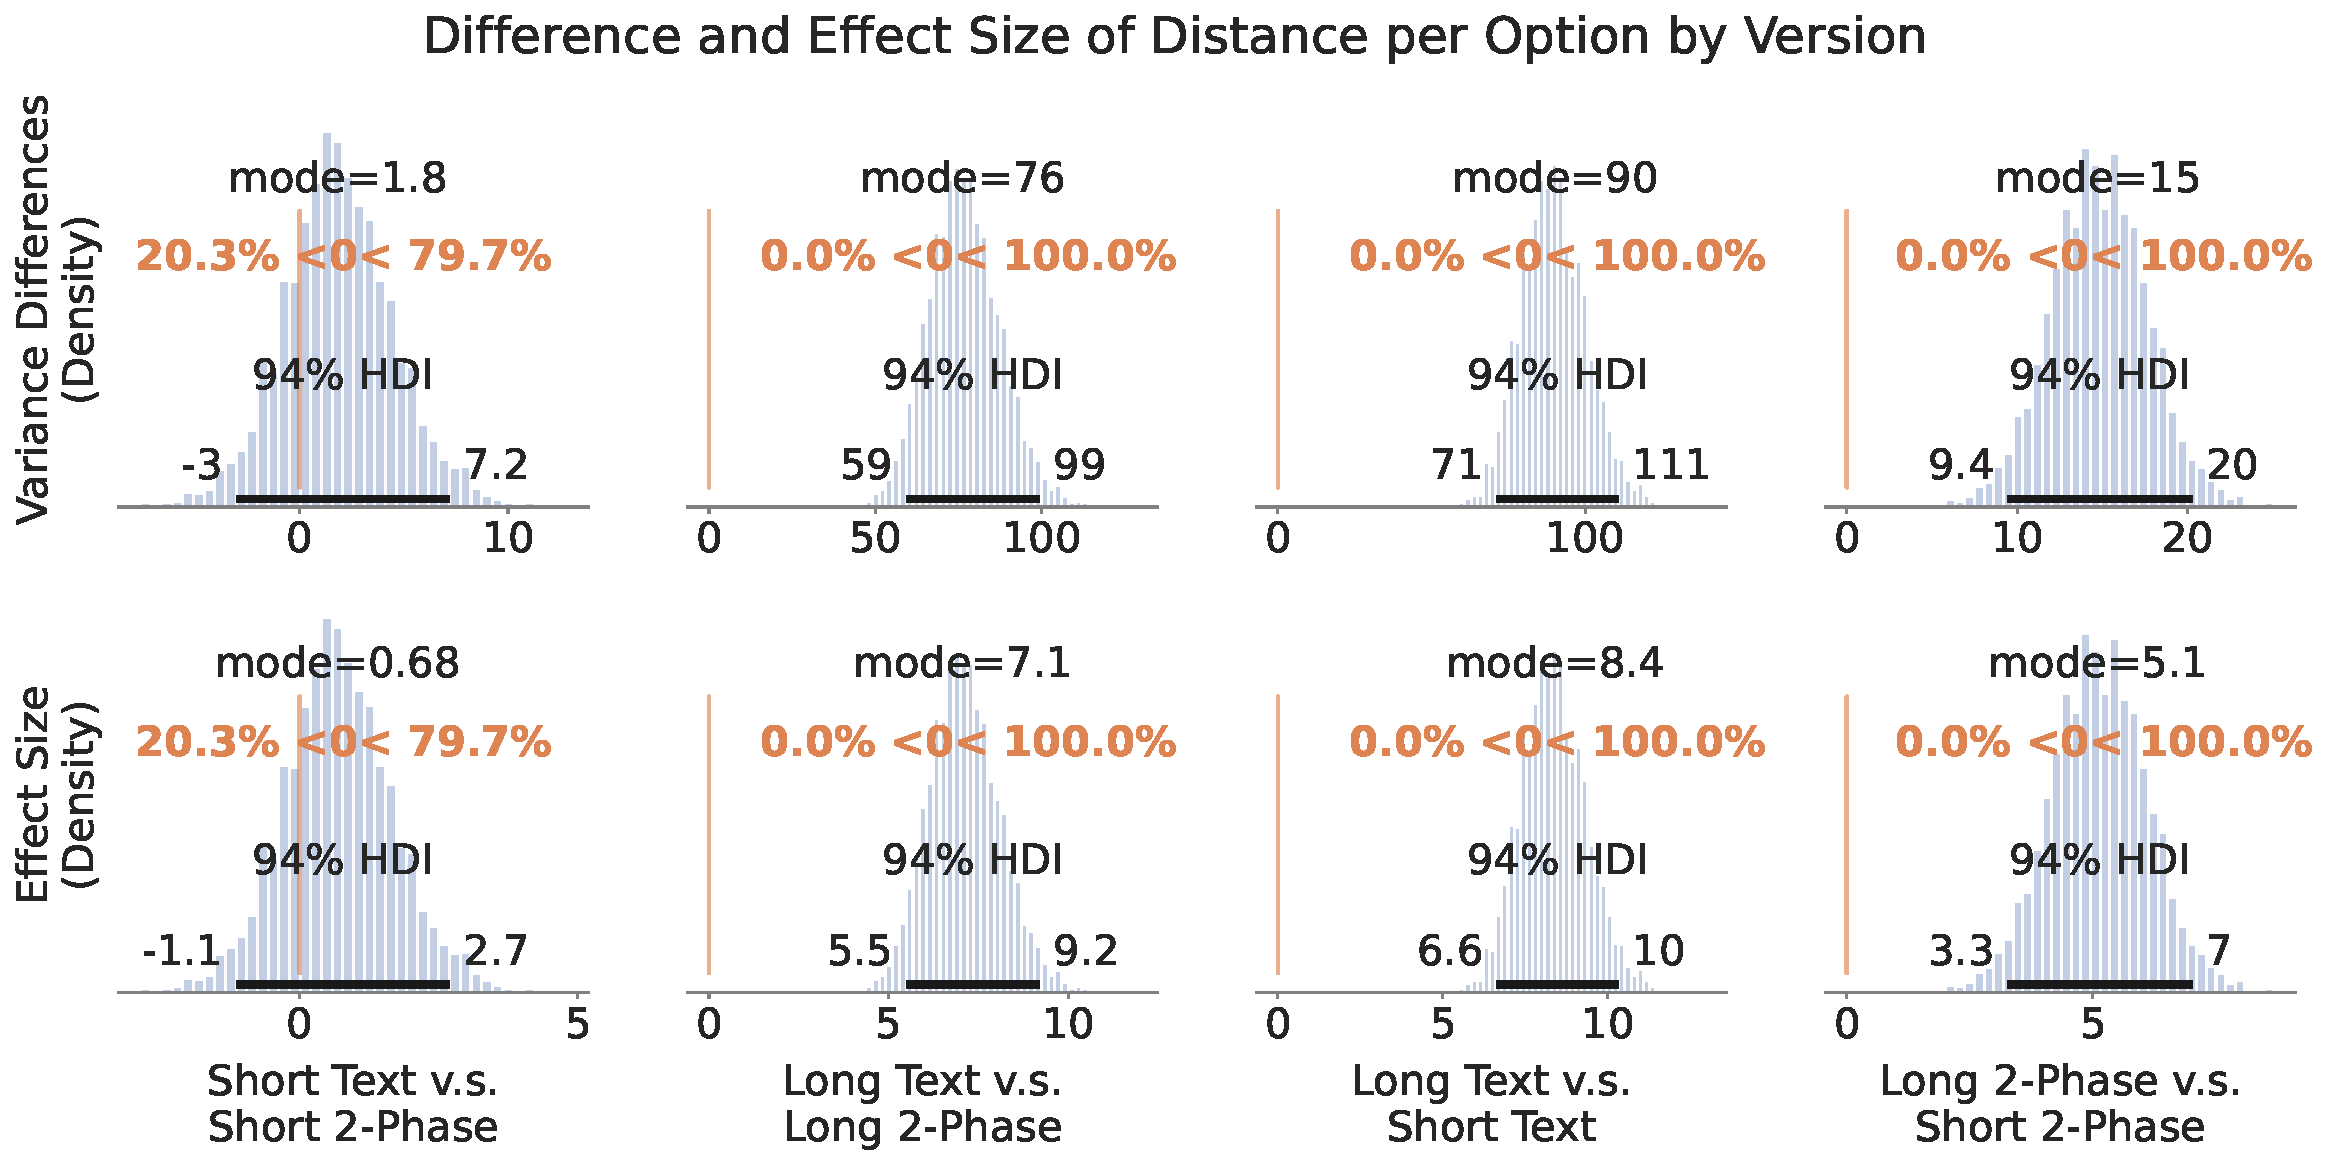
\includegraphics[width=0.8\textwidth]{content/image/distance/distance_diff_per_option_effect_size_by_version_all.pdf}
    \caption{Differences in the variance of edit distance by version.~\textbf{The main takeaway: } In addition to the takaway from the main text, this plot shows that with two-phase interface, there is a reduction is edit distance when the number of option grows.}
    \Description{
    A grid of eight density plots showing the differences and effect sizes of distances per option by version. The top row depicts variance differences, and the bottom row depicts effect sizes, both represented as density distributions. Each column corresponds to a comparison: Short Text vs. Short 2-Phase, Long Text vs. Long 2-Phase, Long Text vs. Short Text, and Long 2-Phase vs. Short 2-Phase. Each plot includes a mode value, a 94\% Highest Density Interval (HDI), and the proportion of the distribution below and above zero. Variance difference distributions on the top row show modes ranging from 1.8 to 90, with varying HDI ranges. Effect size distributions on the bottom row have modes between 0.68 and 8.4, with all 94\% HDIs above zero except for Short Text vs. Short 2-Phase.
    }

    \label{fig:bayesian_distance_variance}
\end{figure*}

\subsubsection{Posterior predictive plots}
Our Bayesian model converged successfully, as evidenced by an $\hat{R}$ value of 1 in the model summary. We plotted the posterior predictive distribution for the edit distance per option in Figure~\ref{fig:observed_vs_posterior_predictive_histogram_m2}. This figure compares the models posterior predictive distribution with the observed data.

\subsubsection{Model Results}
Figure~\ref{fig:bayesian_distance_variance} shows the pairwise comparison of the variance of edit distance in the first row followed by the effect size in the second row. In addition to the comparison within the same survey length, we provide all pairwise comparisons. A notable result that we omit from the main text is that if we compare the variance between the long and short text, and the variance between the long and short two-phase, we see that the text group had three times the standard deviation compared to the two-phase group. This indicates that the organization phase minimize the edit distance despite the increase in survey length.

\subsection{Model 3: Cumulative Edit Distance for long QS} \label{sec:apdx:model_cum_distance}

The dependent variable for this model is the cumulative edit distance $D_i$, a positive continuous variable measured at each step within a version for each user. We modeled this to test our hypothesis that for each participant, the growth rate of the edit distance is consistent. To accommodate its positive nature, we model $D_i$ using a Truncated Normal distribution:

\begin{equation}\label{eq:model3_likelihood}
D_i \sim \text{TruncatedNormal}(\mu_i, \sigma_{\text{obs},i}, \text{lower}=0),
\end{equation}
where the observation-specific standard deviation is given a Half-Normal prior:
\begin{equation}\label{eq:model3_prior_sigma}
\sigma_{\text{obs},i} \sim \text{HalfNormal}(0.3).
\end{equation}

\subsubsection{Independent Variables and Regression Model}
We incorporate the following independent variables: the step number when completing QS ($S_i$), the interface version ($V_i$), and user-specific effects ($U_i$). The interface version and user-specific effects are modeled using hyperpriors to capture variability across groups.

The linear predictor for $D_i$ is given by:
\begin{equation}\label{eq:model3_mu}
    \mu_i = \alpha_{\text{shared}} + \beta_v[V_i] \cdot S_i + U_i \cdot S_i,
\end{equation}
where $\alpha_{\text{shared}}$ represents the global intercept, $\beta_v[V_i]$ models the interface version effects, and $U_i$ captures individual user-specific effects. The intercept is assigned the following prior:
\begin{equation}\label{eq:model3_prior_shared}
    \alpha_{\text{shared}} \sim \mathcal{N}(2.0, 0.5).
\end{equation}

\paragraph{Interface Version ($V_i$).} Interface effects are modeled as:
\begin{equation}\label{eq:model3_prior_beta}
    \beta_v[V_i] \sim \mathcal{N}(\mu_{\beta}, \sigma_{\beta}),
\end{equation}
where the hyperparameters for the interface effect distribution are:
\begin{align}
    \mu_{\beta} &\sim \mathcal{N}(0.05, 0.05), \label{eq:model3_prior_beta_mu}\\
    \sigma_{\beta} &\sim \text{HalfNormal}(0.1). \label{eq:model3_prior_beta_sigma}
\end{align}

\paragraph{User Effects ($U_i$).} Instead of directly sampling $U_i$, we use a reparameterization to mitigate limited user data:
\begin{equation}\label{eq:model3_user_mu}
    U_i = \mu_U + \sigma_U \cdot z_{U,i},
\end{equation}
where $z_{U,i}$ represents individual user variability:
\begin{equation}\label{eq:model3_prior_z}
    z_{U,i} \sim \mathcal{N}(0,1).
\end{equation}
The priors for user effects are:
\begin{equation}\label{eq:model3_prior_user}
    \mu_U \sim \mathcal{N}(0,1), \quad \sigma_U \sim \text{HalfNormal}(0.1).
\end{equation}

\begin{figure}[h!]
    \centering
    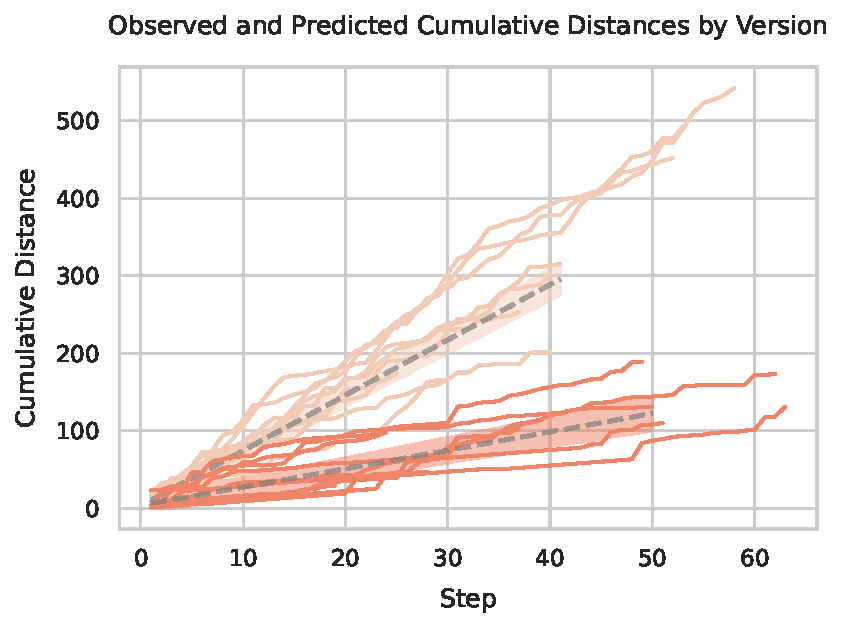
\includegraphics[width=0.45\textwidth]{content/image/distance/observed_and_predicted_cumulative_distances_by_version_m3.pdf}
    \caption{Posterior Predictions vs. observed data for cumulative edit distance. The plot showed each observed user's cumulative edit distance in different shades for the two groups of participants. Dotted line represent the posterior predictive mean. \textbf{Takeaway of the plot}: We believe that the model is reasonable at capturing slop of the cumulative trends.}
    \Description{ A line plot titled "Observed and Predicted Cumulative Distances by Version," showing cumulative distances across task steps for two conditions. Solid lines in varying shades of red and orange, representing actual cumulative distances for individual participants. Dashed lines, showing the model's predicted cumulative distances for each condition. The plot indicates alignment between observed and predicted trends, with some variability at higher cumulative distances. Predictions closely follow observed trajectories, demonstrating the model's accuracy in capturing cumulative distance patterns.}
    \label{fig:observed_and_predicted_cumulative_distances_by_version_m3}
\end{figure}

\subsubsection{Posterior Predictive Plots}

Our Bayesian model converged successfully, as indicated by an $\hat{R}$ value of 1 in the model summary. Figure~\ref{fig:observed_and_predicted_cumulative_distances_by_version_m3} presents the posterior predictive distribution for cumulative edit distance, demonstrating alignment between the predicted and observed data.

\clearpage